\chapter{Metodologia}
    \label{chap:Metodologia}

Este capítulo confere os principais detalhamentos de cunho metodológicos, que guiam as várias etapas desse trabalho, com destaque para \nameref{ClassificacaoPesquisa}, \nameref{PesquisaBibliografica} como método investigativo, \nameref{KanbanAdaptado} como método de desenvolvimento, \nameref{PesquisaAcao} como método de análise de resultados, o \nameref{Fluxo} para realizaçao do TCC 1 e TCC 2, e \nameref{Cronograma} de execução do trabalho. Por fim, têm-se o \nameref{ResumoCap}.



%%%%%%%%%%%%%%%%%%%%%%%%%%%%%%%%%%%%%%%%%%%%%%%%%%%%

\section{Classificação da Pesquisa}
    \label{ClassificacaoPesquisa}

Segundo \cite{ProjPesquisaGil}, uma pesquisa pode ser descrita como um procedimento sistemático e racional destinado a fornecer soluções de problemas. Isso é necessário quando a informação disponível é insuficiente para abordar a questão ou quando essa informação se encontra tão desorganizada que não pode ser adequadamente relacionada ao problema em questão. A condução da pesquisa requer a integração de conhecimentos existentes e a aplicação meticulosa de métodos, técnicas e outros procedimentos científicos. 

A pesquisa desenvolve-se ao longo de um processo composto por várias etapas, desde a formulação adequada do problema até a apresentação satisfatória dos resultados. Dessa forma, todo estudo científico tem início com a colocação de um problema viável, e em seguida inicia a busca por oferecer uma solução potencial, por meio de uma proposição, uma expressão verbal passível de ser comprovada como verdadeira ou falsa. Existem diversas motivações que justificam a realização de uma pesquisa, divididas geralmente em dois grandes conjuntos: motivos de ordem intelectual e motivos de ordem prática. Os primeiros derivam do desejo de adquirir conhecimento por sua própria gratificação. Os últimos têm origem no interesse de obter conhecimento para aprimorar a eficiência ou eficácia em uma determinada área \cite{ProjPesquisaGil}.

Com objetivo de desenvolver a pesquisa deste trabalho da maneira correta diante da determinado questão de problema, há a necessidade de se classificar a pesquisa no que se refere à abordagem, à natureza, aos objetivos e aos procedimentos.

\setfloatlocations{quadro}{hbtp}
\begin{quadro}
\caption{\label{ClassificacaoPesquisTCC}Classificação da Pesquisa}
\centering

\begin{tabular}{|l|l|}
\hline
\textbf{Categoria}     & \textbf{Classificação}                \\ \hline
\textbf{Abordagem}     & Qualitativa                           \\ \hline
\textbf{Natureza}      & Aplicada                              \\ \hline
\textbf{Objetivo}      & Exploratória                          \\ \hline
\textbf{Procedimentos} & Pesquisa Bibliográfica, Pesquisa-ação \\ \hline
\end{tabular}

\legend{Fonte: Autora}
\end{quadro} 

A abordagem deste trabalho é definida como, predominantemente, Qualitativa. Isso ocorre, pois serão utilizadas heurísticas de usabilidade de \citeonline{NNGroupUI}, as quais são coletadas e analisadas de modo subjetivo, uma vez que consideram a experiência individual dos usuários em relação à interface de um sistema. Adicionalmente, ainda visando avaliar a experiência de usuário, mantém-se o viés de abordagem qualitativa, com o uso do Questionário AttrakDiff-R \cite{AttrakDiff}. Nesse caso, é verdade que se tem o uso de números concretos, na escala de 7 pontos likert, o que remete à algo de cunho quantitativo, mas no fundo, a intenção do questionário é avaliar métricas de qualidade, mantendo, predominantemente, a tendência qualitativa do estudo. Detalhes sobre essas métricas inerentes ao Questionário \textit{AttrakDiff-R}, encontram-se esclarecidos no \hyperref[chap:ReferencialTeorico]{Capítulo 2 - Referencial Teórico}, seção \ref{adiff}.

A natureza deste trabalho é classificada como Aplicada. Sendo assim, a finalidade é desenvolver conhecimentos através de aplicação prática, concentrando-se na solução de problemas específicos, e fornecendo soluções sobre o objeto em análise. Nesse sentido, o objetivo é a implantação de melhorias, orientadas à experiência de usuário, na interface de uma típica plataforma de comércio eletrônico móvel, que tenha maior circulação e popularidade entre os usuários, enquanto compram e vendem produtos e serviços. Essa implantação demandará modelagem de protótipos de alta fidelidade em ferramenta especializada, além de levantamento sobre as principais dificuldades encontras pelos usuários ao usarem a plataforma, e a associação entre essas dificuldades e as heurísticas de usabilidade centradas na experiência de usuário.

A pesquisa deste trabalho é classificada como Exploratória. De acordo com \citeonline{ProjPesquisaGil}, essas pesquisas buscam fornecer uma compreensão mais aprofundada do problema para torná-lo mais evidente ou para desenvolver hipóteses. Pode-se afirmar que o principal propósito do presente trabalho é investigar, pesquisar, visando aperfeiçoar ideias e/ou descobrir novas intuições. Isso ocorre no domínio de comércio eletrônico móvel, sendo esse acessado por diferentes tipos de dispositivos, com variadas características, procurando pesquisar se há impactos na experiência dos usuários. Em havendo, e sendo os mesmos impactos negativos, como mitigá-los usando heurísticas estabelecidas na literatura especializada.

Em termos de procedimentos, este trabalho faz uso de Pesquisa Bibliográfica e Pesquisa-ação. A Pesquisa Bibliográfica está sendo utilizada para o levantamento de referências teóricas por meio de bases de científicas. Segundo \citeonline{PesquisaAcaoTripp}, Pesquisa-ação é um processo cíclico, com o objetivo de proporcionar um melhoramento continuado, mesclando investigação e prática. Assim, ocorre planejamento, implementação, descrição e avaliação, visando melhorias contínuas. Detalhes, tanto sobre Pesquisa Bibliográfica, quanto Pesquisa-ação, são apresentados adiante, ainda nesse capítulo, seções \ref{PesquisaBibliografica} e \ref{PesquisaAcao}.

%%%%%%%%%%%%%%%%%%%%%%%%%%%%%%%%%%%%%%%%%%%%%%%%%%%%

\section{Pesquisa Bibliográfica}
\label{PesquisaBibliografica}

Para elaboração deste trabalho, tem sido necessário realizar levantamentos com base em materiais da literatura especializada relacionados aos tópicos de interesse, sendo: domínio de comércio eletrônico móvel, experiência de usuário e heurísticas de usabilidade. A ideia é conferir uma base de conhecimento, que permita compreender de forma mais adequada sobre o contexto do trabalho como um todo, além de fundamentar as colocações apresentadas ao leitor dessa monografia.

Até o momento, foram utilizadas três bases cientificas para a realizar a pesquisa de materiais bibliográficos, sendo: Scielo, IEEE e Google Acadêmico. Nessas plataformas, foram utilizadas as \textit{strings} de busca: \textit{e-commerce, m-commerce, user experience} e \textit{AttrakDiff}.

Foram priorizados os termos em inglês, pois são conferidos muito mais referências e fontes, se comparado aos retornos conferidos com base nos termos em português. Esse quantitativo maior permite realizar uma pesquisa mais abrangente. Os próprios materiais escritos em português, comumente, referenciam os termos em inglês, sendo possível encontrar materiais escritos em português no retorno da busca.

A Tabela \ref{StringBase} resume, para cada \textit{string} de busca, e combinação das mesmas, o quantitativo de materiais retornados.

\begin{table}[]
\caption{\label{StringBase}Quantitativo de materiais retornados com as strings de busca}
\centering
\begin{tabular}{l|l|l}
\hline
\textit{String}                   & Base de Dados                                                           & Quantidade \\ \hline
"user experience" AND "e-commerce" & Google Acadêmico                                                        & 32,473     \\ \hline
"user experience" AND "m-commerce" & Google Acadêmico                                                        & 17.500     \\ \hline
"user experience" AND "AttrakDiff" & Google Acadêmico                                                        & 3.230      \\ \hline
"user experience" AND "e-commerce" & IEEE                                                                    & 345        \\ \hline
"user experience" AND "e-commerce" & ScienceDirect (Elsevier) & 3,192      \\ \hline
\end{tabular}
\legend{Fonte: Autora}
\end{table}

Como foram retornados vários materiais, ocorreu a necessidade de ter critérios de seleção, visando separar materiais mais aderentes ao perfil de interesse do presente trabalho.

Os critérios utilizados para seleção dos artigos foram:
\begin{itemize}
    \item Ter sido escrito em português, inglês, alemão;
    \item O resumo ter termos chave relacionados aos tópicos de interesse deste trabalho, e
    \item Apresentar métricas relacionadas a Comércio Eletrônico (\textit{e-commerce}), Comércio Móvel (\textit{m-commerce}), Experiência de Usuário e Usabilidade.
\end{itemize}

Tendo estes critérios como base de seleção, os principais materiais que embasam o trabalho são: \cite{SudianaChandra}, \cite{LucasAlmeida}, \cite{GunawanRicky}, \cite{ECommerceOverview} e \cite{AttrakDiff}.

Percebe-se que há materiais mais antigos, mas que são muito bem referenciados na área de Interação Humano-Computador e afins. Há ainda materiais de 2021, que conferem maior atualidade ao trabalho. De toda forma, já tem um tempo que as áreas de interesse vêm contribuindo com guias de boas práticas para se ter adequada experiência de usuário. Entretanto, de acordo com uma pesquisa prévia realizada até o momento nesse trabalho, percebe-se que as plataformas de comércio eletrônico ainda não implantam essas práticas na íntegra. Acredita-se que muito se deva à necessidade de desenvolvimento rápido dessas plataformas, para não perder mercado para os concorrentes. Afinal, desenvolver com cuidado, e de forma atenciosa, demanda tempo. Tempo, no meio comercial, á algo que custa muito caro para as empresas. 

Diante do exposto, um propósito a ser atingido nesse trabalho é justamente conferir um estudo que mostre as principais dificuldades encontradas pelos usuários, que afetam a experiência desses usuários, mesmo considerando uma plataforma muito popular e associada a um grande \textit{player} do domínio de comércio eletrônico móvel. Com isso, prototipar algumas telas, conferindo um olhar da literatura, que acorda heurísticas de usabilidade, orientadas à experiência de usuário, e que mitigam tais dificuldades.


\section{Kanban Adaptado}
    \label{KanbanAdaptado}

Trata-se do método utilizado por esse trabalho para condução de diferentes etapas, que vão desde a escolha do tema, às pesquisas investigativa, aplicada e avaliativa, culminando na apresentação os membros da banca.

O Kanban é um sistema visual de gestão de trabalho que utiliza um quadro com colunas para acompanhar o progresso das tarefas. Cada tarefa é representada por um cartão, movendo-se de uma coluna para outra conforme avança no processo. O sistema limita o número de tarefas em andamento em cada etapa, mantendo o foco e evitando sobrecarga. Os cartões devem conter informações básicas sobre a atividade, como descrição, prazo e responsável. Em geral, o quadro é dividido em seções como  \textit{ToDo} (Para fazer), \textit{Doing} (Fazendo) e \textit{Done} (Feito) \cite{Kanban}.

Na Figura \ref{kanban}, tem-se um exemplo do Quadro Kanban, com as colunas que orientam o fluxo de trabalho de \textit{ToDo}, \textit{Doing} e \textit{Done}.

\begin{figure}[ht]
    \centering
    \caption{Exemplo de uso do Quadro Kanban}
    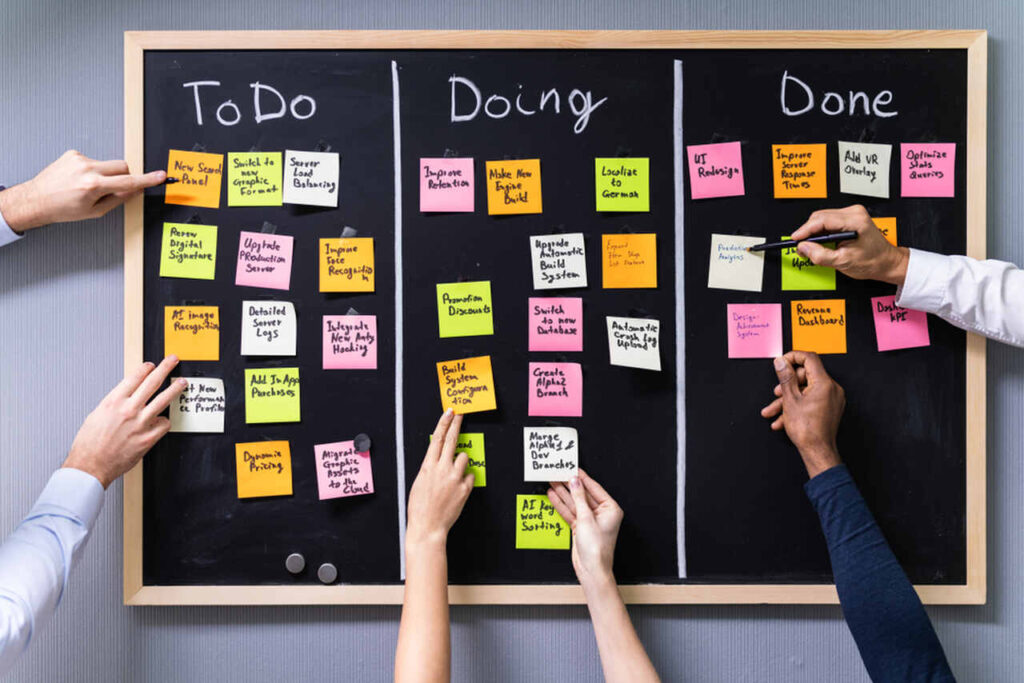
\includegraphics[keepaspectratio=true,scale=1.2]{figuras/kanban.jpg}
    \legend{Fonte: \cite{Kanban}}
    \label{kanban}
\end{figure}

Para cada etapa do trabalho, serão criados cartões específicos centrados em tarefas, em um primeiro momento, na coluna \textit{ToDo}. Ao ser colocado em execução, o cartão será arrastado para a coluna \textit{Doing}. Por fim, ao ser concluída a tarefa prevista no cartão, o mesmo será arrastado para a coluna \textit{Done}, finalizando o processo. Isso permitirá manter o controle sobre cada etapa do trabalho.

As principais etapas do trabalho são expostas na Figura \ref{kanbanmeu}, para o caso do TCC (primeira parte):

\begin{figure}[ht]
    \centering
    \caption{Etapas Primeira Parte TCC em Kanban}
    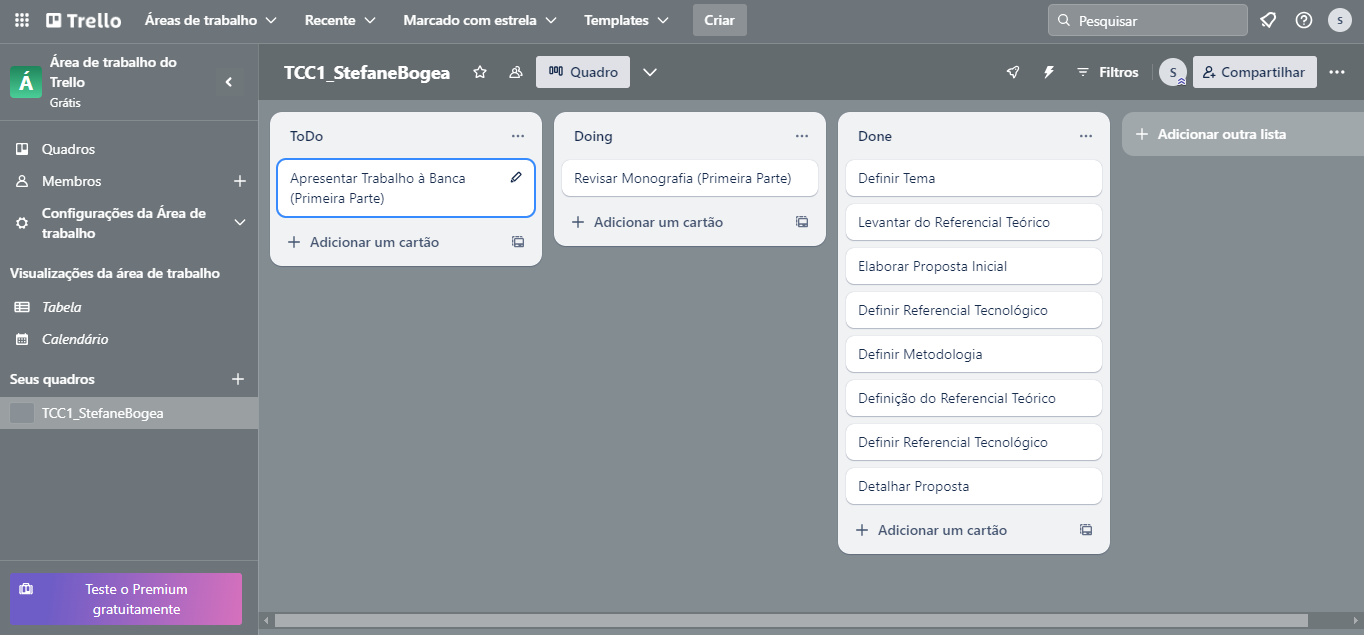
\includegraphics[keepaspectratio=true,scale=0.4]{figuras/kanbanmeu.png}
    \legend{Fonte: Autora}
    \label{kanbanmeu}
\end{figure}

%%%%%%%%%%%%%%%%%%%%%%%%%%%%%%%%%%%%%%%%%%%%%%%%%%%%

\section{Pesquisa-ação}
 \label{PesquisaAcao}

A pesquisa-ação destaca-se em relação a outros métodos de pesquisa. Essa diferença não é apenas pela flexibilidade, mas também, e principalmente, devido à integração da ação dos pesquisadores e dos grupos envolvidos. Esta integração acontece em várias fases ao longo do processo de pesquisa, indo além dos elementos tradicionais de uma pesquisa convencional \cite{ProjPesquisaGil}. As etapas da pesquisa-ação são: fase exploratória, formulação do problema, construção de hipóteses, realização do seminário, seleção da amostra, coleta de dados, análise e interpretação dos dados, elaboração do plano de ação e divulgação dos resultados. Tendo em vista a condução da pesquisa deste trabalho, as etapas previstas são:

\begin{itemize}
    \item Coleta de Dados: Esta etapa consiste no levantamento de informações através de questionários. Em um primeiro momento, visando identificar quais são as plataformas mais conhecidas no domínio de comércio eletrônico móvel, elegendo uma como exemplo. Em um segundo momento, com o uso do questionário AttrakDiff-R, com o objetivo de identificar as principais dificuldades encontradas pelos usuários ao usar essa plataforma exemplo, com foco na experiência do usuário.
    \item Análise e Interpretação dos Dados: Com o levantamento de dados realizado, será possível analisar os resultados obtidos, a fim de entender quais são as dificuldades dos usuários em uma típica plataforma de comércio eletrônico móvel, de acordo com as métricas estabelecidas pelo questionário AttrakDiff-R. Com base na literatura e considerando as dificuldades identificadas, pretende-se associar as boas praticas de usabilidade, listadas pelas Heurísticas de Nielsen, e essas dificuldades.
    \item Elaboração do Plano de Ação: Com a análise dos dados concluída, inicia-se o plano de ação. Nesse caso, tem-se a elaboração de protótipos de alta fidelidade utilizando a plataforma Figma, e visando mostrar de forma clara como é possível mitigar os erros encontrados aplicando as boas práticas de usabilidade. Espera-se, com isso, que o nível de satisfação em termos de experiência de usuário seja maior.
    \item Divulgação dos Resultados: Com a finalização de cada uma das etapas da pesquisa-ação, todo o processo será documentado como parte dos resultados deste Trabalho de Conclusão de Curso como parte da conclusão da segunda parte.
\end{itemize}

%%%%%%%%%%%%%%%%%%%%%%%%%%%%%%%%%%%%%%%%%%%%%%%%%%%%

\section {Fluxo de Atividades}
\label{Fluxo}

Para elaboração deste trabalho foi necessário a divisão de atividades detalhadas para melhor desenvolvimento de cada etapa do estudo. As principais etapas do trabalho essão expostas na Figura \ref{fig06}, para o caso do TCC 1:

\begin{figure}[ht]
    \centering
    \caption{Etapas Primeira Parte TCC}
    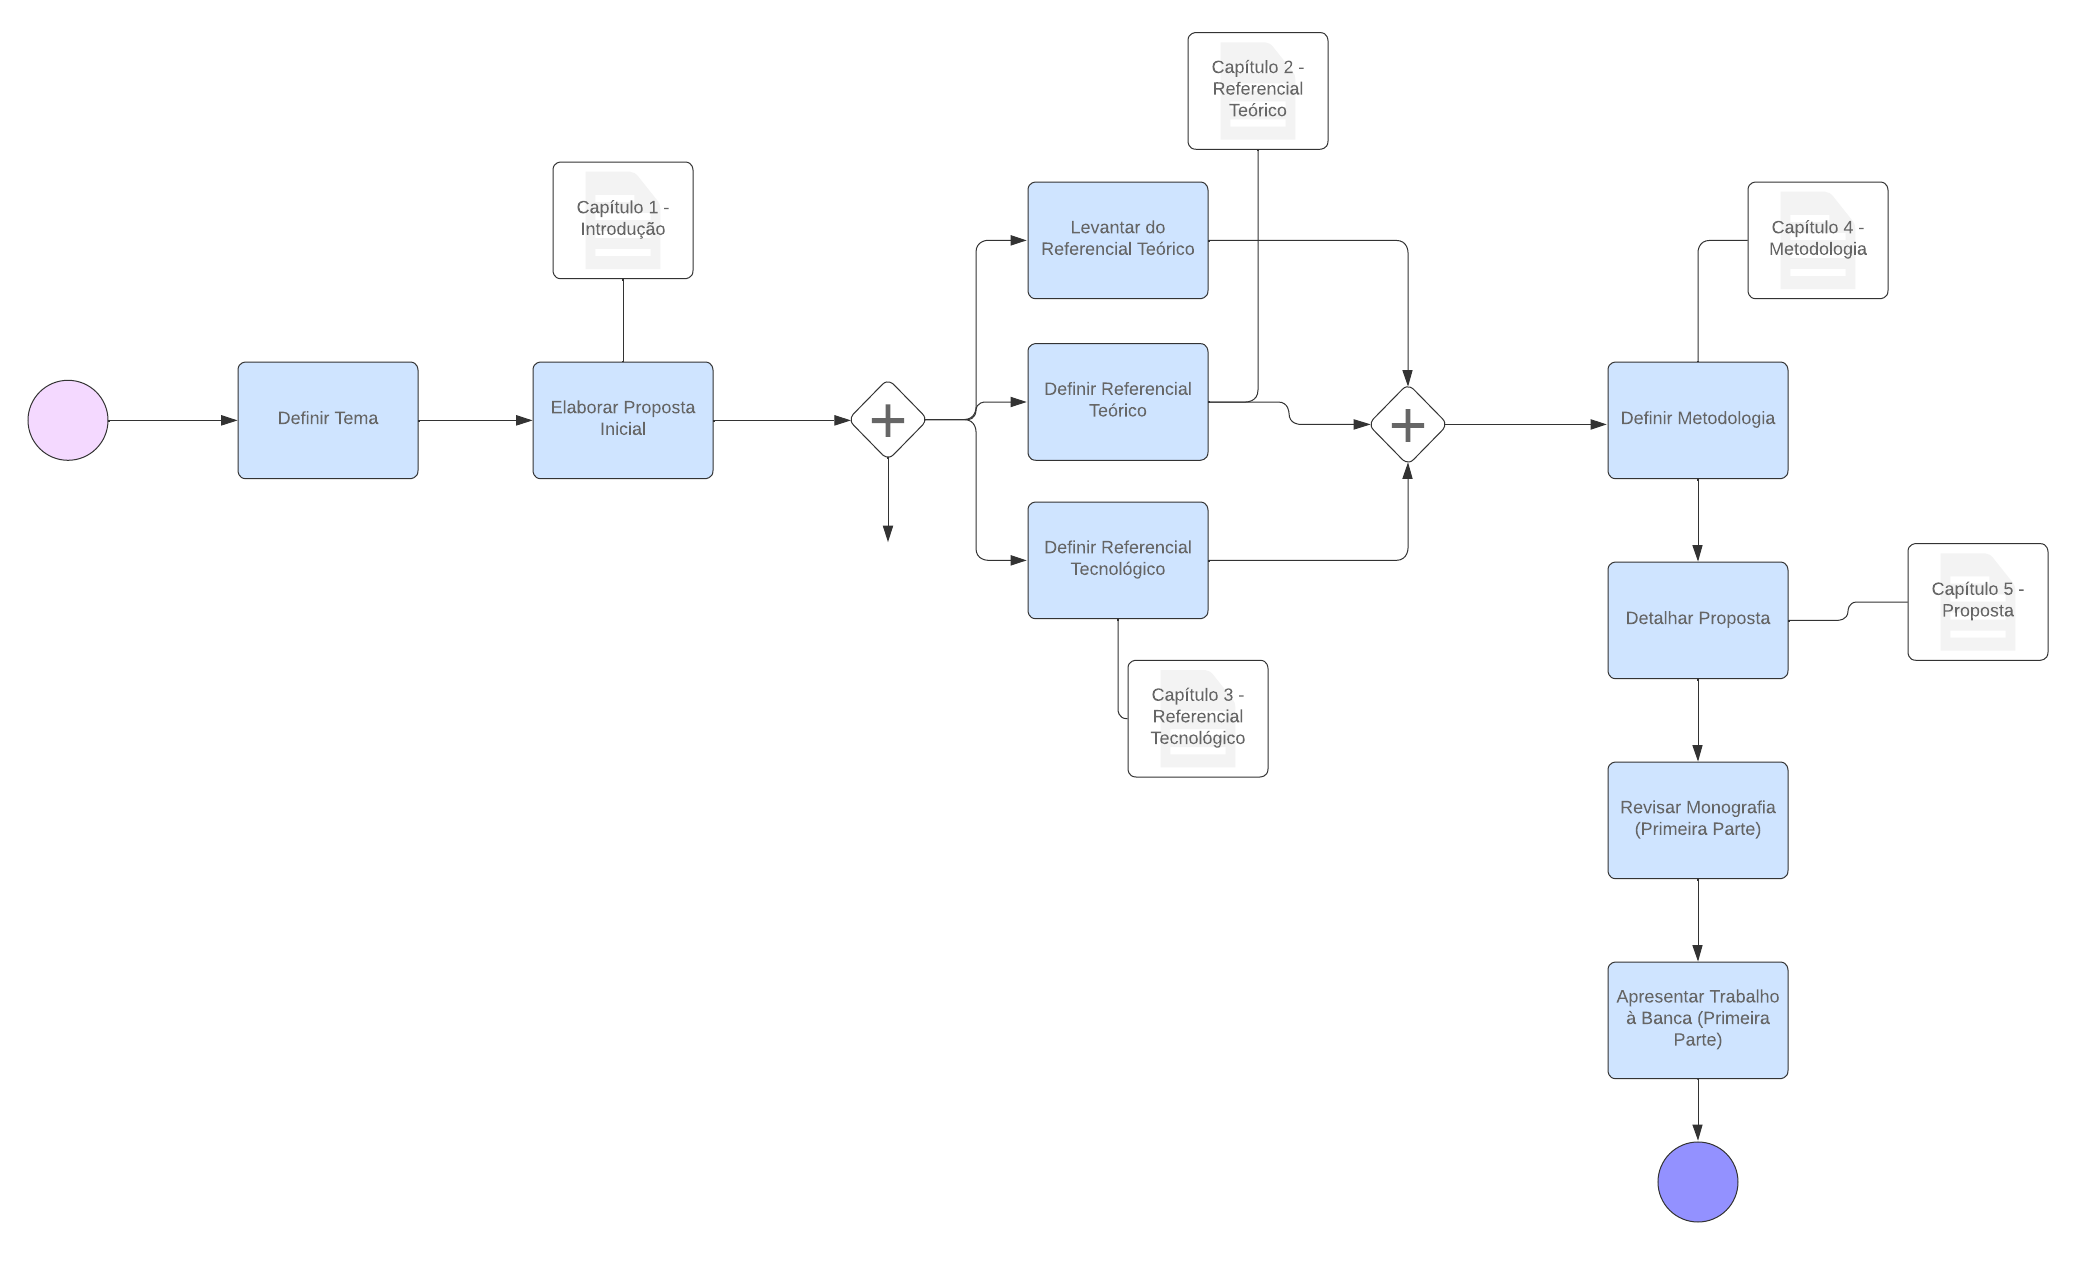
\includegraphics[keepaspectratio=true,scale=0.2]{figuras/cap04Fluxograma1.png}
    \legend{Fonte: Autora}
    \label{fig06}
\end{figure}

\textbf{Definir Tema}: Tarefa que foi cumprida no intuito de estabelecer um foco de estudo a ser explorado no trabalho, resultando no tema resumido no título dessa monografia.

\textbf{Levantar do Referencial Teórico}: Tarefa que foi concluída com o objetivo de realizar um levantamento do referencial teórico buscando identificar, revisar e analisar as teorias, conceitos e estudos relevantes que fornecem embasamento teórico para sua investigação.

\textbf{Elaborar Proposta Inicial}: Tarefa que tem como objetivo definir a proposta do estudo mediante a literatura encontrada estabelecendo os objetivos finais do trabalho, cujos encontram-se no \hyperref[chap:Introducao]{Capítulo 1 - Introdução}.

\textbf{Definição do Referencial Teórico}: Subprocesso que compreendeu: (i) levantar os principais materiais de apoio junto às bases científicas, orientando-se pelo método investigativo Pesquisa Bibliográfica, descrita anteriormente, e (ii) documentação sobre os tópicos de interesse investigados, cujos resultados encontram-se no \hyperref[chap:ReferencialTeorico]{Capítulo 2 - Referencial Teórico}.

\textbf{Definir Referencial Tecnológico}: Tarefa que, com base nos tópicos teóricos definidos no subprocesso anterior, resultou na escrita do \hyperref[chap:ReferencialTeorico]{Capítulo 3 - Referencial Tecnológico}. Têm-se, portanto, os principais suportes que apoiam a pesquisa, o desenvolvimento e outros aspectos complementares desse trabalho. Há destaque para a ferramenta Figma, a ser utilizada para prototipagem das melhorias na interface da plataforma de comércio eletrônico móvel exemplo. Além disso, cabe mencionar o uso do AttrakDiff-R, para análise dos feedbacks dos usuários, orientando-se pela perspectiva da experiência de usuário.

\textbf{Definir Metodologia}: Tarefa que compreendeu a Classificação da Pesquisa, bem como a definição dos métodos investigativo (Pesquisa Bibliográfica); de desenvolvimento (Kanban Adaptado) o fluxo de atividades para as duas etapas do trabalho e de análise de resultados (Pesquisa-Ação). Como resultado dessa tarefa, tem-se o presente o \hyperref[chap:Metodologia]{Capítulo 4 - Metodologia}. 

\textbf{Detalhar Proposta}: Tarefa visando descrever de forma mais detalhada a proposta, resultando na escrita do \hyperref[chap:Proposta]{Capítulo 5 - Proposta}.

\textbf{Revisar Monografia (Primeira Parte)}: Tarefa que ocorreu em paralelo a todas as demais, sendo demandada sempre que uma versão mais avançada da monografia era obtida.

\textbf{Apresentar Trabalho à Banca (Primeira Parte)}: Tarefa a ser realizada em breve, visando mostrar o trabalho aos membros da banca, recebendo e anotando seus pontos de vista.

Na segunda parte do TCC, Figura \ref{fig07}, estão previstas as seguintes etapas:

\begin{figure}[ht]
    \centering
    \caption{Etapas Segunda Parte TCC}
    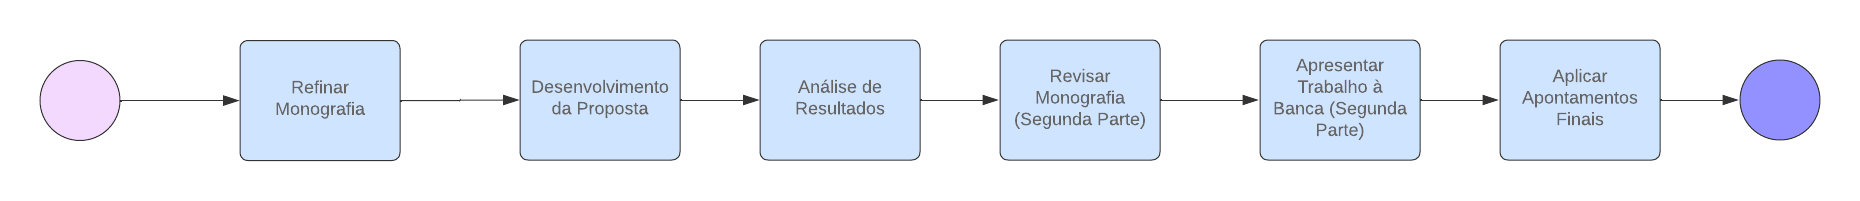
\includegraphics[keepaspectratio=true,scale=0.2]{figuras/cap04Fluxograma2.png}
    \legend{Fonte: Autora}
    \label{fig07}
\end{figure}

\textbf{Refinar Monografia}: Tarefa que consistirá em refinar a monografia, conforme apontamentos dos membros da banca.

\textbf{Desenvolvimento da Proposta}: Subprocesso que coloca em prática as demais subtarefas inerentes aos objetivos específicos desse trabalho, com destaque para a Identificação das principais dificuldades encontradas pelos usuários ao interagirem com plataformas de comércio eletrônico móvel; e a associação entre as dificuldades identificadas e as principais técnicas/práticas de usabilidade orientadas à experiência de usuário. Aqui, será utilizado o Kanban Adaptado, já explicado anteriormente.

\textbf{Análise de Resultados}: Subprocesso que compreende, principalmente, a realização das etapas prevista na Pesquisa-ação, visando a aplicação de melhorias - prototipagem - em uma plataforma de comércio eletrônico móvel, com base na associação obtida com o cumprimento do subprocesso anterior "Desenvolvimento da Proposta". Outros detalhes desse método de análise de resultados podem ser consultados em Pesquisa-ação, mais adiante nesse capítulo.

\textbf{Revisar Monografia (Segunda Parte)}: Tarefa que ocorrerá em paralelo a todas as demais, sendo demandada sempre que uma versão mais avançada da monografia for obtida.

\textbf{Apresentar Trabalho à Banca (Segunda Parte)}: Tarefa a ser realizada, visando mostrar o trabalho final aos membros da banca, recebendo e anotando seus pontos de vista.

\textbf{Aplicar Apontamentos Finais}: Tarefa que compreende a realização de refinamentos, orientando-se pelos apontamentos da banca, e visando obter a versão final da monografia.

%%%%%%%%%%%%%%%%%%%%%%%%%%%%%%%%%%%%%%%%%%%%%%%%%%%%

\section{Cronograma}
    \label{Cronograma}

Com base no fluxo de atividades abordado que foi acordada, foi elaborado um cronograma a ser seguido durante o desenvolvimento da primeira parte do TCC, como mostrado no Quadro \ref{Cronograma1}, e o cronograma para o desenvolvimento da segunda parte TCC, como mostrado no Quadro \ref{Cronograma2}.

\setfloatlocations{quadro}{hbtp}
\begin{quadro}
\caption{\label{Cronograma1}Cronograma da Primeira Parte do TCC}
\centering

\begin{tabular}{|p{7cm}|p{1.5cm}|p{1.5cm}|p{1.5cm}|p{1.5cm}|p{1.5cm}|}
\hline
\textbf{Atividade} & \textbf{Nov/23} & \textbf{Dez/23} & \textbf{Jan/24} & \textbf{Fev/24} & \textbf{Mar/24} \\ \hline
{Definir Tema} & X &  &  &  &  \\ \hline
{Levantar do Referencial Teórico} &  & X &  &  &  \\ \hline
{Elaborar Proposta Inicial} &  & X &  &  &  \\ \hline
{Definição do Referencial Teórico} &  & X &  & X &  \\ \hline
{Definir Referencial Tecnológico} &  &  &  & X &  \\ \hline
{Definir Metodologia} &  & X &  &  &  \\ \hline
{Detalhar Proposta} &  &  &  & X &  \\ \hline
{Revisar Monografia} &  &  &  & X & X \\ \hline
{Apresentar Trabalho} &  &  &  &  & X \\ \hline
\end{tabular}

\legend{Fonte: Autora}
\end{quadro} 

\setfloatlocations{quadro}{hbtp}
\begin{quadro}
\caption{\label{Cronograma2}Cronograma da Segunda Parte do TCC}
\centering

\begin{tabular}{|p{7cm}|p{1.5cm}|p{1.5cm}|p{1.5cm}|p{1.5cm}|p{1.5cm}|}
\hline
\textbf{Atividade} & \textbf{Mar\textbackslash{}24} & \textbf{Abr/24} & \textbf{Mai/24} & \textbf{Jun/24} & \textbf{Jul/24} \\ \hline
{Correções Sugeridas pela Banca} & X &  &  &  &  \\ \hline
{Desenvolvimento} &  & X &  &  &  \\ \hline
{Atualização dos Caps. 1, 2, 3 e 4} &  & X & X &  &  \\ \hline
{Desenvolvimento} &  &  & X &  &  \\ \hline
{Análise de Resultados} &  &  & X & X &  \\ \hline
{Abordagem Desenvolvida} &  &  &  & X &  \\ \hline
{Análise de Resultados} &  &  &  & X &  \\ \hline
{Conclusão} &  &  &  & X &  \\ \hline
{Finalização Geral da Monografia} &  &  &  &  & X \\ \hline
\textbf{Apresentação à Banca} &  &  &  &  & X \\ \hline
\end{tabular}

\legend{Fonte: Autora}
\end{quadro} 

%%%%%%%%%%%%%%%%%%%%%%%%%%%%%%%%%%%%%%%%%%%%%%%%%%%%

\section{Resumo do Capítulo}
    \label{ResumoCap}

Este capítulo ofereceu uma visão geral em termos metodológicos, destacando alguns métodos que sustentam este estudo. A pesquisa foi classificada, segundo os critérios: abordagem (predominantemente, Qualitativa), natureza (Aplicada), objetivo (Exploratória) e procedimentos (Pesquisa Bibliográfica e Pesquisa-ação). O método de desenvolvimento concentra-se no uso do Quadro Kanban. Já o método de  análise de resultados abrange a Pesquisa-ação, acordando sobre suas principais etapas. Constam ainda detalhamentos sobre os fluxos de tarefas/subprocessos, bem como cronogramas, tanto para o escopo da primeira etapa, quanto para o escopo da segunda etapa desse trabalho.

